\input xy
\xyoption{all}
\documentclass{beamer}
\usepackage{amsmath,latexsym,amssymb,mathrsfs,graphicx}
\newtheorem {conclusion}                  [theorem]{Conclusion}
\newcommand {\FF}                         {\mathcal{F}}
\newcommand {\W}                          {\mathcal{W}}
\newcommand {\G}                          {\mathcal{G}}
\newcommand {\A}                          {\mathcal{A}}
\newcommand {\B}                          {\mathcal{B}}
\newcommand {\N}                          {\mathbb{N}}
\newcommand {\C}                          {\mathbb{C}}
\newcommand {\R}                          {\mathcal{R}}
\newcommand {\X}                          {\Xi}
\newcommand {\x}                          {\xi}
\newcommand {\f}                          {\varphi}
\newcommand {\p}                          {\psi}
\newcommand {\m}                          {\mu}
\newcommand {\rr}                         {\varrho}
\newcommand {\pp}                         {\varpsi}
\newcommand {\lL}                         {\lambda}
\newcommand {\LL}                         {\Lambda}
\newcommand {\noi}                        {\noindent}
\newcommand {\spaces}                     {\,\,\,}
\def\labelenumi{(\alph{enumi})}
\def\theenumi{\alph{enumi}}
\graphicspath{ {./images/} }
%Information to be included in the title page:
\title{Formal Concept Analysis, Lattice Polinomials and Approximation}
\author{Levan Tsinadze}
\institute{Tbilisi State University}
\date{2022}

\begin{document}

\frame{\titlepage}

\begin{frame}
    \frametitle{Why Formal Concept Analysis}
    \begin{figure}
        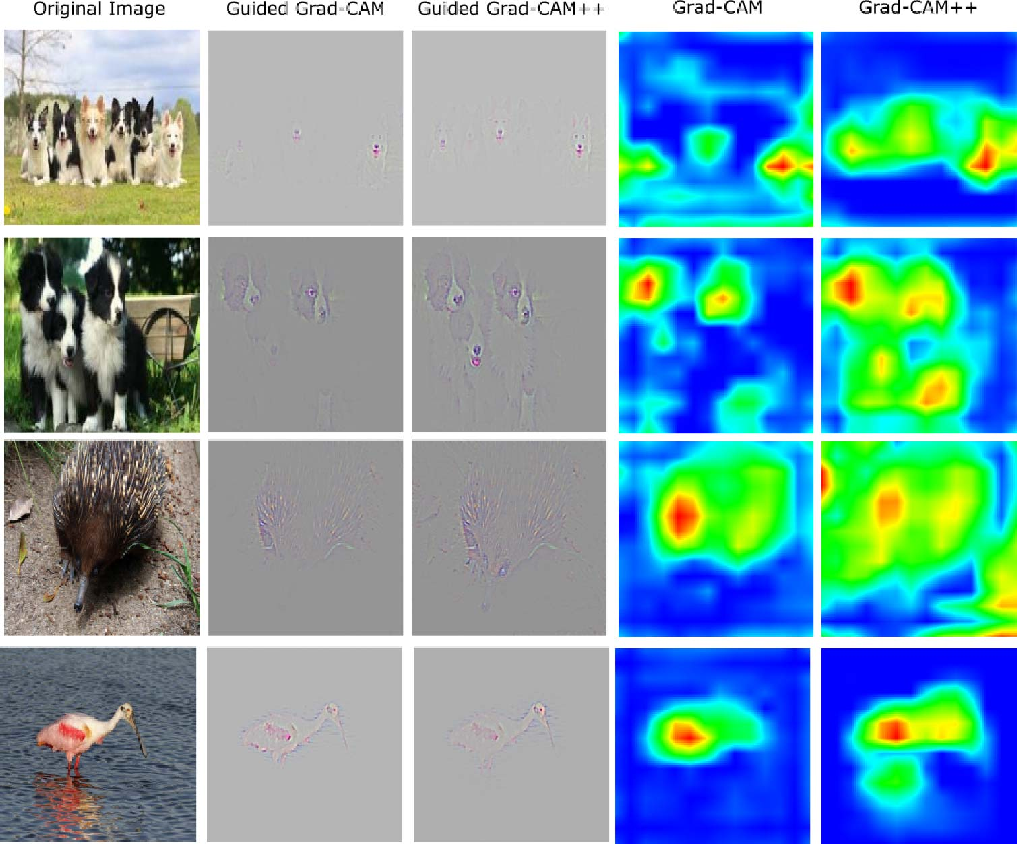
\includegraphics[width=\linewidth]{grad_cam_1.png}
        \caption{Common and hiuerarchical features}
        \label{fig:gradcam}
      \end{figure}
\end{frame}

\begin{frame}
    \frametitle{Aggregation of Common Features}
    \begin{figure}
        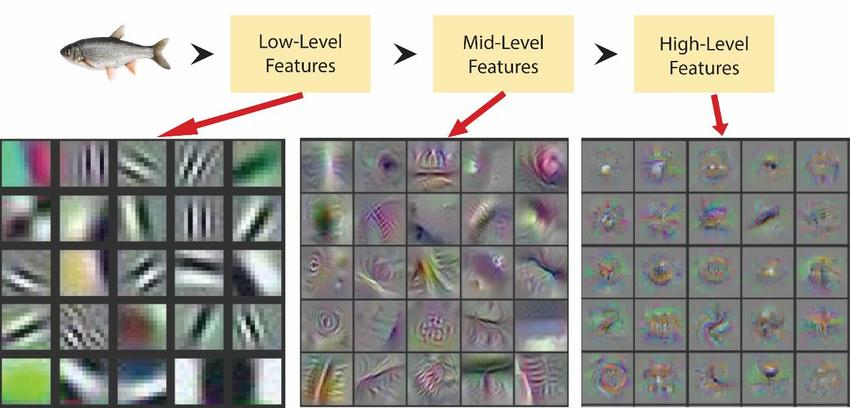
\includegraphics[width=\linewidth]{hierarchical_aggr.png}
        \caption{Hierarchical Aggregation of Features}
        \label{fig:hieragr}
      \end{figure}
\end{frame}

\begin{frame}
    \frametitle{Concept Partial Order}
        As it is defined in \cite{FCATut}:
        \begin{itemize}
            \item Formal Context is a triple $(G, M, I)$ 
            where $G$ and $M$ are sets and $I \subset G \times M$ 
            is a relation betweeen them which is callsed incidence relation, 
            $G$ is called objects and $M$ attributes 
            \item For subset of objects $A \subset G$  define 
            $A' =\{ m\in M | (g, m) \in I \text{ for all }g \in A \}$
            \item For subset of attributes $B \subset M$ define
            $B' =\{ g\in G | (g, m) \in I \text{ for all } m \in B \}$
            \item A concept of the context $(G, M, I)$ is apair $(A, B)$ 
            where $A \subset G$, $B \subset M$ with properties $A' = B$ and $B' = A$
            \item For two concepts $(A_1,B_1)$ and $(A_2,B_2)$ define order 
            $(A_1,B_1) \le (A_2,B_2)  \iff A_1 \subset A_2  \iff B_1 \subset B_2$
        \end{itemize}
\end{frame}

\begin{frame}
    \frametitle{Example of Concepts}
    \begin{figure}
        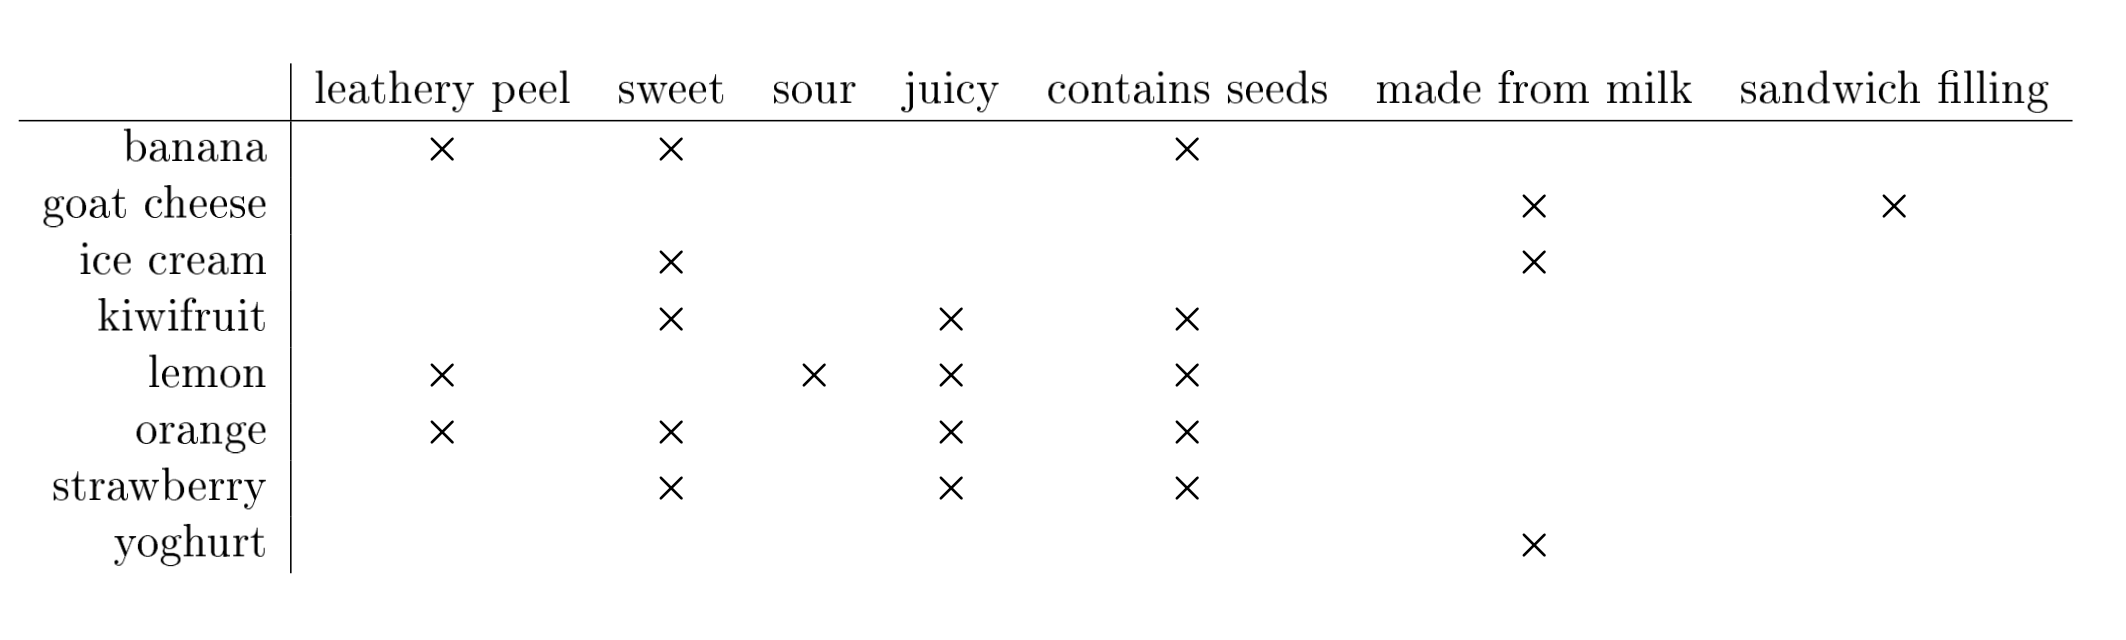
\includegraphics[width=\linewidth]{concept_1.png}
        \caption{Incidence Table of Fruits.}
        \label{fig:fruits}
      \end{figure}
\end{frame}

\begin{frame}
    \frametitle{Hesse Diagram of Concepts}
    \begin{figure}
        \centering
        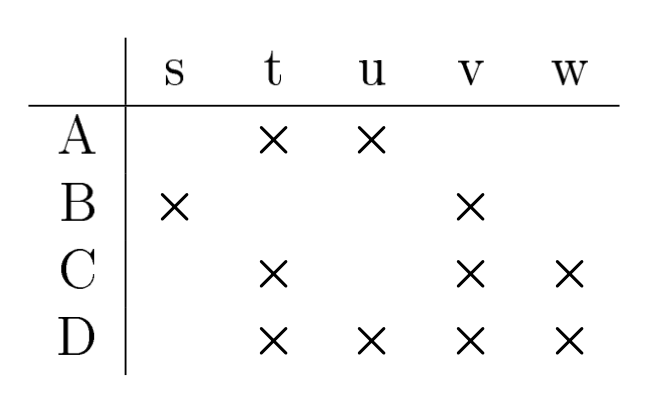
\includegraphics[width=0.4\linewidth]{cross_table_2.png} 
        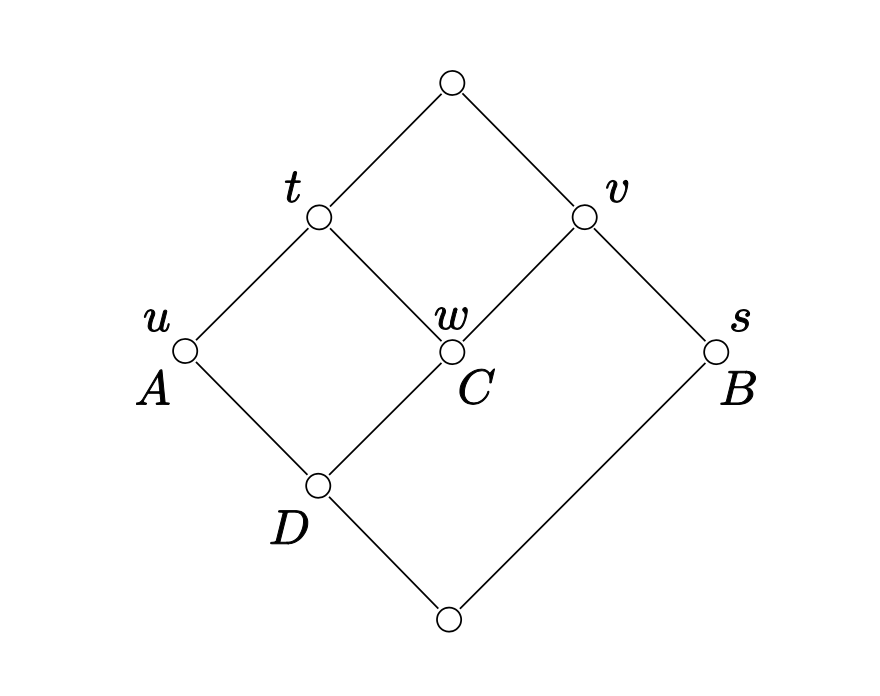
\includegraphics[width=0.4\linewidth]{hesse_diagram_1.png}
        \caption{Cross-table and Hesse Diagram}
        \label{fig:cross_table_hesse_diag}
    \end{figure}
        
    Context with order might be visualized an Hesse diagram
\end{frame}

\begin{frame}
    \frametitle{Concept Lattice}
    Denote set of all concepts on context $(G, M, I)$ as $\B(G, M I)$

    Then it is easy to proofe that $\B(G, M I)$ is complete lattice with meet and join
    operations:
    $$
    \bigvee_{j \in J}{(A_j, B_j)} = ((\bigcup_{j \in J}{A_j})', \bigcap_{j \in J}{B_j})
    $$
    and
    $$
    \bigwedge_{j \in J}{(A_j, B_j)} = (\bigcap_{j \in J}{A_j}, (\bigcup_{j \in J}{B_j})')
    $$
    With this we can refine context or reduce it, 
    or find appropriate attributes for class of objects for clusterization, classification, 
    knowledge discovery, etc.
\end{frame}

\begin{frame}
    \frametitle{Formal Concept Analysis and Decision Trees}
    If we consider objects as in our dataset and attributes as features, we can define
    analysis of machine learning model and find similarities with formal concept analysis
    an machine learning architectures
    \begin{itemize}
        \item In \cite{ClassFCA} defined several methods for classification using 
        Formal Concept Analysis
        \item In \cite{DesTreeLatt}, \cite{DesRFCL}, \cite{LattClassTree} Formal Concept Analysis
        is applied for decision tree classification and found different concept classification rules
        also conversion of lattice to the decision trees
    \end{itemize}
\end{frame}

\begin{frame}
    \frametitle{Piecewise Appriximation Functions}
    In \cite{NNCPWLRepr} neural networks are defined as 
    continous piecewise linear functions and representation of each finity pieces 
    continous piecewise linear functions with neural netwoeks established. Which gives 
    isomorphic functor $F : \mathbb{NN} \to \mathbb{CPWL}$ among categories of neural networks 
    and continous piecewise linear functions.

    For piecewise approximation defined on $X$ as 
    $\FF :X \times P \to Y$ where for each $p \in P$ projection is basis:
    $$\left.\FF\right|_{X \times \{p\}} = \f : X \to Y$$
    we can define $\B \subset 2^X$ as 
    pieces or batches for which approximation happens on one particular basis function.
    
    Define $\A = (\A, \le)$ partially ordered set and  $\alpha : \FF \times 2^{X} \to \A$ 
    which maps each pair $(\f, B) = \f(B)$ to the single approximation $A \in \A$
    \begin{itemize}
        \item For each $B \in \B$ approximation happens on one particular basis function $\f$
        \item $\cup {\B} = X$
    \end{itemize}
    For instance linear regresion or neural network as piecewise universal approximator
    for $l_2$ or $l_1$ with $\A = \mathbb{R}_+$
\end{frame}

\begin{frame}
    \frametitle{Spetwise Approximation}
    \begin{figure}
        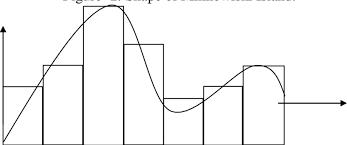
\includegraphics[width=\linewidth]{step_approx_1.png}
        \caption{Step by step approximation (MLP).}
        \label{fig:stepapp}
    \end{figure}
\end{frame}

\begin{frame}
    \frametitle{Priecwise Linear Approximation}
    \begin{figure}
        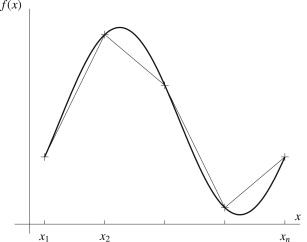
\includegraphics[width=\linewidth]{cpwl_approx_1.jpg}
        \caption{Continous priecewise linear approximation (ReLU).}
        \label{fig:cpwlapp}
    \end{figure}
\end{frame}

\begin{frame}
    \frametitle{Sigmoid Approximation}
    \begin{figure}
        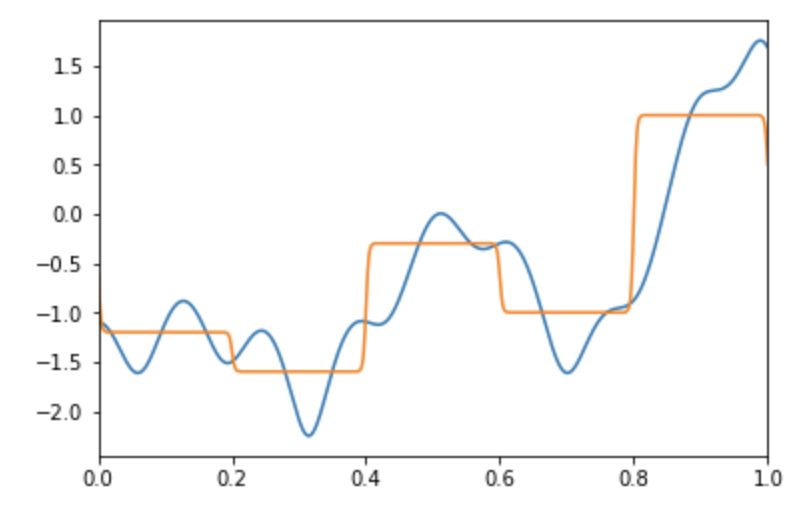
\includegraphics[width=\linewidth]{sig_approx_1.jpeg}
        \caption{Piecewise continous nonlinear approximation (Sigmoid).}
        \label{fig:sigapp}
    \end{figure}
\end{frame}

\begin{frame}
    \frametitle{Piecewise linear / continous piecewise linear function as lattice polinomials}
    Consider pairs $(\f, B)$ on batches and rder:
    \begin{itemize}
        \item $(\f, B) \le (\f, D)$ if $\alpha(\f(B)) \le \alpha(\f(D)) \iff B \subset D$
        \item $\f(x) \land \p(y) = \m(\{x, y\})$ where $\f, \p$ and $\m$ are basis of $\FF$ 
    \end{itemize}
    Of course $\land$ operation is defined with respect to $\A$ and it is more categorical 
    limit which is unique up to isomorphism
\end{frame}

\begin{frame}
    \frametitle{Data Fitting on Two Items}
    \begin{figure}
        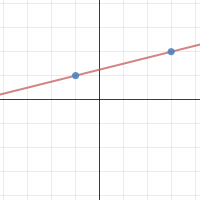
\includegraphics[width=\linewidth]{linear_two_1.png}
        \caption{Approximation on two points.}
        \label{fig:lintwo}
    \end{figure}
\end{frame}

\begin{frame}
    \frametitle{Data Fitting on Two Items}
    \begin{figure}
        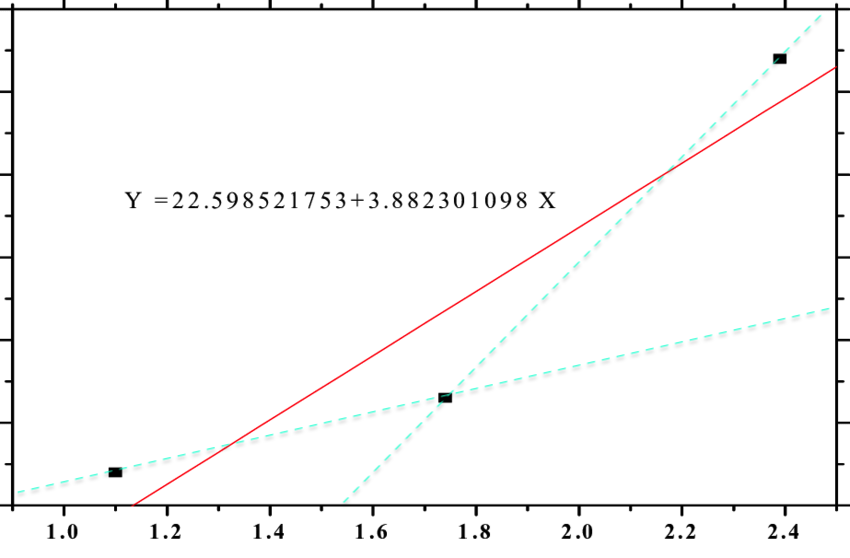
\includegraphics[width=\linewidth]{linear_three_1.png}
        \caption{Approximation on three points.}
        \label{fig:linthree}
    \end{figure}
\end{frame}

\begin{frame}
    \frametitle{The Best Approximation Batches}
    Consider pairs $(\f, B)$ on batches and order:
    \begin{itemize}
        \item $\bigwedge_{\f \in \FF}{(\f(B))}$
        \item $\bigvee_{B \in \B}{(\f, B)}$
    \end{itemize}
    This gives the best approximation batches $\B$ for $\FF$ function and $\A$ approximation.
\end{frame}

\begin{frame}
    \frametitle{Lattice Polinomial and Formal Concept}
    So we can consider neural network, linear regression and multi-linear regressions as:
    \begin{description}
        \item[1] $K(B) = \bigwedge_{\f \in \FF}{\f(B)}.$ fitting on batch
        \item[2] $K(\A, \FF) = \bigvee_{B \in \B}{K(B)}$ fitting on functions
        where $\f(x) \lor \p(x) = \max{(\alpha(\f(x)), \alpha(\p(x)))}$ as in \cite{PWLRegConf},
        \cite{PWLLattMinp1} and \cite{PWLLattMinp2} but towards approximation.
    \end{description}

\end{frame}

\begin{frame}
    \frametitle{Hierarchical Lattice Polinomials}
        If we define refinement of $\B^{l}$ by the $B^{l+1}$:
        \begin{description}
            \item[1] For each $B^{l} \in \B^{l}$ there exists $B^{l + 1} \in \B^{l + 1}$
            such that $B^{l + 1} \subset B^{l}$
            \item[2] For each $B^{l} \in \B^{l} $ we have 
            $\bigcup_{b^{l + 1} \subset B^{l}}{B^{l + 1}} = B^{l}$
        \end{description}

        We can distinguish layer of the lattice polinomial:
        $$
        K^{l + 1}(\A) = \bigvee_{B^{l+1} \in \B^{l+1}}K^l(B^{l+1})
        $$
\end{frame}

\begin{frame}
    \frametitle{Representation Learning}
    For later layers we can investigate lattice polinomial of this layer:
    $$
    K^{l + 1}(\A)
    $$

    If we fix the layer $l$ we can consider approximation / representation power
    of the appropriated polinomial
\end{frame}

\begin{frame}
    \frametitle{Further Work 1}
    Investigate lattice polinomial and learning objective 
    along with natural topology / metric / (quasi) uniform structures 
    on $X$ and $Y$ spaces
    \begin{itemize}
        \item Investigate model capacity by amount of batches 
        and memorization capacity \cite{RandLabs} 
        \item Investigation if kernel machines can be represented as a lattice polinomials
        \item Compare lattice polinomials of different models and analysis of similarities
        \cite{NNKernalMach}, \cite{NNKerLearn}
        \item Investigate overparametrization \cite{NNOverparam}
        \item Self-supervised representation learning and transfer learning 
        as lattice polinomials \cite{PerSal}, \cite{PanYang}, \cite{FurZhan}, \cite{ChenKorbin},
        \cite{HeWe}, \cite{OordLi}, \cite{GrillFlor}, \cite{DevlChang}, \cite{LiuOtt},
        \cite{VelicFedus}, \cite{GroverLesk}, \cite{KipfWell}, \cite{ZhuXu}, \cite{LiuZhang}, 
        \cite{JaisBabu}, \cite{XieXu}, \cite{WuLin}, \cite{YouChen}, \cite{ThakCor}.
        \item Investigate (uniformly) continous property for each lattice polinomial
        \item Compact and locally compact structures
    \end{itemize}
\end{frame}

\begin{frame}
    \frametitle{Further Work 2}
    \begin{itemize}
        \item Completness and completion of $X$ and $Y$ spaces
        \item Tropical geometry of machine learning and deep learning 
        \cite{MaragCharTheod}, \cite{ZhNaitLim}
        \item Analysis on generalization capaciry and overfitting
    \end{itemize}
    Whole area for research.
\end{frame}

\begin{frame}
    \frametitle{Thank You}
\end{frame}

\begin{frame}
    \frametitle{Questions}
\end{frame}

\begin{frame}
    \frametitle{Thank You Angain}
\end{frame}

\begin{thebibliography}{...}
    \bibitem{FCATut} B. Ganter, R. Wille, Formal Concept Analysis: Mathematical Foundations, 
    Springer-Verlag Berlin/Heidelberg/New York, 1999.

    \bibitem{ClassFCA} N. Meddouri, M. Maddouri, Classification Methods based on Formal Concept Analysis,
    Conference: Concept Lattices and their ApplicationsAt: Olomouc, Czech Republic

    \bibitem{DesTreeLatt} R. Belohlavek, B. De Baets, J. Outrata, V. Vychodil, Inducing decision trees via concept lattices,
    International Journal of General Systems, volume 38, 2009 - Issue 4: Concept-lattice applications

    \bibitem{DesRFCL} E. Dudyrev, S. O. Kuznetsov, Decision Concept Lattice vs. Decision Trees and Random Forests,
    arXiv:2106.00387

    \bibitem{LattClassTree} László Kovács, Generating decision tree from lattice for classification,
    Proceedings of the 7th International Conference on Applied Informatics
    Eger, Hungary, January 28-31, 2007. Vol. 2. pp. 377-384.

    \bibitem{PWLRegConf} J.M. Tarela and M.V. Martinez, Region configurations for realizability of lattice
    piecewise-linear models, Mathematical and Computer Modelling, 30(1999), 17-27

    \bibitem{PWLLattMinp1} J.M. Tarela, J.M. Pérez, V. Aleixandre, Minimization of lattice polynomials on piecewise linear functions
    (Part I)
    Annales de l'Association Internationale pour le Calcul Analogique (2) (1975), pp. 79-85

    \bibitem{PWLLattMinp2} J.M. Tarela, J.M. Pérez, V. Aleixandre, Minimization of lattice polynomials on piecewise linear functions
    (Part II)
    Annales de l'Association Internationale pour le Calcul Analogique (2) (1975), pp. 121-127

    \bibitem{NNKernalMach} P. Domingos, Every Model Learned by Gradient Descent Is Approximately a Kernel Machine,
    arXiv:2012.00152

    \bibitem{NNKerLearn} A. Jacot, F. Gabriel, C. Hongler, Neural Tangent Kernel: Convergence and Generalization in Neural Networks,
    arXiv:1806.07572

    \bibitem{NNOverparam} S. S. Du, X. Zhai, B. Poczos, A. Singh, Gradient Descent Provably Optimizes Over-parameterized Neural Networks,
    arXiv:1810.02054

    \bibitem{RandLabs} C. Zhang, S. Bengio, M. Hardt, B. Recht, O. Vinyals, Understanding deep learning requires rethinking generalization,
    arXiv:1611.03530

    \bibitem{NNCPWLRepr} J. He, L. Li, J. Xu, C. Zheng, ReLU Deep Neural Networks and Linear Finite Elements,
    arXiv:1807.03973v2

    \bibitem{MLPUA} K. Hornik, M. Stinchcombe and H. White, Multilayer feedforward networks are
    universal approximators, Neural networks, 2(1989), 359-366.

    \bibitem{ONELayerUA} G. Cybenko, Approximation by superpositions of a sigmoidal function, 
    Mathematics of control, signals and systems, 2(1989), 303-314.

    \bibitem{MaragCharTheod} P. Maragos; V. Charisopoulos; E. Theodosis, Tropical Geometry and Machine Learning,
    Proceedings of the IEEE, Volume: 109 Issue: 5

    \bibitem{ZhNaitLim} L. Zhang, G. Naitzat, L. H. Lim, Tropical Geometry of Deep Neural Networks,
    arXiv:1805.07091

    \bibitem{AdaHerStr} J. Ad\'amek, H. Herrlich and G.E. Strecker, Abstract and concrete
    categories,
    Wiley Interscience, New York, 1990.
    
    \bibitem{Bru} G.C.L. Br\'ummer, Categorical aspects of the theory of
    quasi-uniform spaces, Rend. Ist. Mat. Univ. Trieste 30 Suppl., 1999,
    45-74.
    
    \bibitem{FleLin} P. Fletcher and W.F. Lindgren, Quasi-uniform spaces, Lecture
    Notes Pure Appl. Math. 77, Dekker, New York, 1982.
    
    \bibitem{FleLinn} P. Fletcher and W.F. Lindgren, Locally quasi-uniform spaces with
    countable bases, Duke Math. J. 41, 1971, 369-372.
    
    \bibitem{HinHuf} T.L. Hincks and S.M. Huffuman, A note on locally quasi-uniform
    spaces, Canad. Math. Bull. Vol. 19(4), 1976, 501-504.
    
    \bibitem{Mac} S. Mac Lane, Categories for the working mathematician,
    Springer-Verlag, New York-Heidelberg-Berlin, 1971.
    
    \bibitem{TsinSev} L. Tsinadze, Several types of locally quasi-uniform spaces and their
    categories, functorial local quasi-uniformities, in preparation.
    
    \bibitem{TsinEpir} L. Tsinadze, Epireflection of completion of 
    localy quasi-uniform spaces, in preparation.
    
    \bibitem{Wil} J. Williams, Locally uniform spaces, Transactions of the American
    Mathematical Society, Volume 168, 1972, 435-469.
    
    \bibitem{PerSal} D.N. Perkins and G. Salomon, Transfer of Learning. 
    Oxford, England: Pergamon, 1992. 

    \bibitem{PanYang} S.J. Pan and Q. Yang, A survey on transfer learning, 
    IEEE Trans. Knowl. Data Eng., vol. 22, no. 10, pp. 1345–1359, Oct. 2010.

    \bibitem{FurZhan} Fuzhen Zhuang, Zhiyuan Qi, Keyu Duan, Dongbo Xi, Yongchun Zhu, 
    Hengshu Zhu, Senior Member, IEEE, Hui Xiong, Fellow, IEEE, and Qing HeA, 
    Comprehensive Survey on Transfer Learning

    \bibitem{ChenKorbin} Ting Chen, Simon Kornblith, Mohammad Norouzi, 
    and Geoffrey E. Hinton. 
    A simple framework for contrastive learning of visual representations. 
    arXiv preprint arXiv:2002.05709, 2020.

    \bibitem{HeWe} Kaiming He, Haoqi Fan, Yuxin Wu, Saining Xie, and Ross 
    B. Girshick. 
    Momentum contrast for unsupervised visual representation learning. 
    arXiv preprint arXiv:1911.05722, 2019

    \bibitem{OordLi} Aäron van den Oord, Yazhe Li, and Oriol Vinyals. 
    Representation learning with contrastive predictive coding. 
    arXiv preprint arXiv:1807.03748, 2018.
                            
    \bibitem{GrillFlor} Jean-Bastien Grill, Florian Strub, 
    Florent Altché, Corentin Tallec, Pierre H. Richemond, Elena Buchatskaya, 
    Carl Doersch, Bernardo Avila Pires, Zhaohan Daniel Guo, 
    Mohammad Gheshlaghi Azar, Bilal Piot, Koray Kavukcuoglu, 
    Rémi Munos, Michal Valko, 
    Bootstrap your own latent: A new approach to self-supervised Learning

    \bibitem{GoodBeng} Ian Goodfellow, Yoshua Bengio, Aron Courvile, 
    Deep Learning

    \bibitem{DevlChang} Jacob Devlin, Ming-Wei Chang, Kenton Lee, 
    Kristina Toutanova, 
    BERT: Pre-training of Deep Bidirectional Transformers for Language Understanding

    \bibitem{LiuOtt} Yinhan Liu, Myle Ott, Naman Goyal, Jingfei Du, Mandar Joshi, 
    Danqi Chen, Omer Levy, Mike Lewis, Luke Zettlemoyer, Veselin Stoyanov, 
    RoBERTa: A Robustly Optimized BERT Pretraining Approach

    \bibitem{VelicFedus} Petar Veličković, William Fedus, William L. Hamilton, 
    Pietro Liò, Yoshua Bengio, R Devon Hjelm, 
    Deep Graph Infomax

    \bibitem{GroverLesk} A. Grover and J. Leskovec, 
    “node2vec: Scalable feature learning for networks,” in SIGKDD, 2016, pp. 855–864. 

    \bibitem{KipfWell} T. N. Kipf and M. Welling, 
    “Variational graph auto-encoders,” in NeurIPS Workshop, 2016, pp. 1-3. 

    \bibitem{ZhuXu} Y. Zhu, Y. Xu, F. Yu, Q. Liu, S. Wu, and L. Wang, 
    “Deep Graph Contrastive Representation Learning,” in ICML Workshop, 2020. 

    \bibitem{LiuZhang} X. Liu, F. Zhang, Z. Hou, L. Mian, Z. Wang, J. Zhang, 
    and J. Tang, 
    “Self-supervised learning: Generative or contrastive,” IEEE TKDE, 2021. 

    \bibitem{JaisBabu} A. Jaiswal, A. R. Babu, M. Z. Zadeh, D. Banerjee, 
    and F. Makedon, 
    “A survey on contrastive self-supervised learning,” 
    Technologies, vol. 9, no. 1, p. 2, 2021. 

    \bibitem{XieXu} Y. Xie, Z. Xu, J. Zhang, Z. Wang, and S. Ji, 
    “Self-supervised learning of graph neural networks: A unified review,” 
    arXiv:2102.10757, 2021.

    \bibitem{WuLin} L. Wu, H. Lin, Z. Gao, C. Tan, S. Li et al., 
    “Self-supervised on graphs: Contrastive, generative, or predictive,” 
    arXiv:2105.07342, 2021. 

    \bibitem{YouChen} Y. You, T. Chen, Y. Sui, T. Chen, Z. Wang, and Y. Shen, 
    “Graph contrastive learning with augmentations,” 
    in NeurIPS, vol. 33, 2020, pp. 5812–5823.

    \bibitem{ThakCor} Shantanu Thakoor, Corentin Tallec, Mohammad Gheshlaghi Azar, 
    Remi Munos, Petar Veličković, Michal Valko, 
    Bootstrapped Representation Learning on Graphs

    \bibitem{Tsin} L. Tsinadze, Universal Representators in Model Spaces, 
    in preparation.
\end{thebibliography}

\end{document}